% ----- Presentation -----

\subsection{Presentation}

    A \textbf{heuristic algorithm} is a type of algorithm that uses criteria to try to find an approximate solution to a problem, rather than an exact one. Heuristic algorithms are often used when it is not possible to find an ideal solution to a problem, or when a perfect solution would be too time-consuming to compute. They are also used when an approximate solution is good enough. Heuristic algorithms are commonly used in artificial intelligence, computer science, and other fields. They are often used to solve optimization problems, search problems, and other types of problems where an exact solution is not necessary or practical.
    \\ \\
    A \textbf{constructive heuristic} algorithm is a type of heuristic algorithm that is used to find a solution to a problem by building it incrementally. Constructive heuristics start with a partial solution and gradually improve it until a complete solution is found.
    \\ \\
    To solve the MEWC with a constructive algorithm, we will need some criteria : 

    \begin{enumerate}
        \item Add a first Vertex to make a partial solution.
        \item Seek for one of his neighbors. And add it to solution if it's a neighbor of all vertices in solution(to be sure to hold a clique in the final result).
        \item Repeat the step 2 until no vertices is available to add
        \item Calculate the weight of the clique found
    \end{enumerate}

    We will then have for solution a maximum clique with his weight. 
    \\ \\
    It is important to define the different criteria in a rigorous way. 
    \\ \\
    The first one is the choice of the first Vertex. Indeed, it is this one which will define the quality of our solution. Taking it randomly would be useless and counter productive for the sake of solving MEWC. As it was important, we thought about how to choose it and 2 answers appeared to us and we have a debate on the subject because we could not reach a consensus on it. We hesitated between these two solutions:

    \begin{itemize}
        \item The first idea was to take the highest degree vertex of the graph given as input. 
        \begin{itemize}
            \item One reason to choose the highest degree vertex as the first vertex in the solution is that it may be more likely to be part of a maximum edge weight clique(because it's the case where it's the most likely to be member of the biggest clique who could be the MEWC). This is because it will allow more edges to be added to the solution, which can increase the overall sum of edge weights in the clique.
            \item Another reason is that it may be more likely to be connected to other high degree vertices. This means that by adding the highest degree vertex to the clique first, we may be able to include other high degree vertices in the clique as well, which can further increase the overall sum of edge weights.
        \end{itemize}
        \item The second one was to take the vertex with the highest sum of weights of the edges.
        \begin{itemize}
            \item One reason to choose the vertex with the highest edge weight as the first vertex in the clique is that it may be more likely to be part of a maximum edge weight clique(because it's the case where it's the most likely to be member of the most weighted clique who could be the MEWC). This is because adding a vertex with a high edge weight to the clique will contribute more to the overall sum of edge weights in the clique, which is what we are trying to maximize.
            \item Moreover, by taking a vertex with adjacent edges of high weight, one is more likely to find adjacent vertices that also have edges of high weight, which increases the probability of finding a clique of maximum weight. On the other hand, taking a vertex with higher degree, one is more likely to find adjacent vertices that have lower weight edges, which decreases the probability of finding a maximum weight clique.
        \end{itemize}
    \end{itemize}
    
    We will illustrate these explanations with figure 11 and 12 which shows the advantages of each over the other.
    \\ \\
    \begin{minipage}{\linewidth}
        \begin{minipage}{0.5\textwidth}
            \begin{figure}[H]
                \centering
                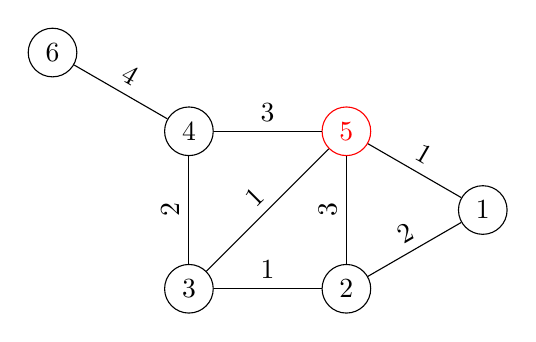
\begin{tikzpicture}[node distance=2cm]
                    \node[circle, draw] (1) {1};
                    \node[circle, draw] (2) at ([shift=(210:2)] 1) {2};
                    \node[circle, draw] (3) [left of=2] {3};
                    \node[circle, draw] (4) [above of=3] {4};
                    \node[circle, draw, red] (5) [above of=2] {5};
                    \node[circle, draw] (6) at ([shift=(150:2)] 4) {6};
    
                    \draw  (1) -- (2) node[midway, above, sloped] {2};
                    \draw (1) -- (5) node[midway, above, sloped] {1};
                    \draw (2) -- (3) node[midway, above, sloped] {1};
                    \draw (2) -- (5) node[midway, above, sloped] {3};
                    \draw (3) -- (4) node[midway, above, sloped] {2};
                    \draw (4) -- (5) node[midway, above, sloped] {3};
                    \draw (4) -- (6) node[midway, above, sloped] {4};
                    \draw (5) -- (3) node[midway, above, sloped] {1};
                \end{tikzpicture}
                \caption{Graph illustration for the highest degree vertex}
                \label{fig:vertex-highest-degree}
            \end{figure}
        \end{minipage}
        \begin{minipage}{0.5\textwidth}
            \begin{figure}[H]
                \centering
                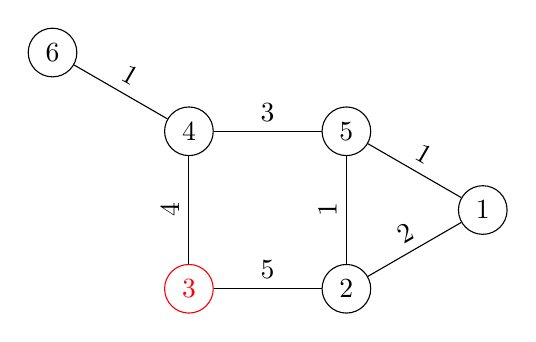
\begin{tikzpicture}[node distance=2cm]
                    \node[circle, draw] (1) {1};
                    \node[circle, draw] (2) at ([shift=(210:2)] 1) {2};
                    \node[circle, draw, red] (3) [left of=2] {3};
                    \node[circle, draw] (4) [above of=3] {4};
                    \node[circle, draw] (5) [above of=2] {5};
                    \node[circle, draw] (6) at ([shift=(150:2)] 4) {6};
    
                    \draw  (1) -- (2) node[midway, above, sloped] {2};
                    \draw (1) -- (5) node[midway, above, sloped] {1};
                    \draw (2) -- (3) node[midway, above, sloped] {5};
                    \draw (2) -- (5) node[midway, above, sloped] {1};
                    \draw (3) -- (4) node[midway, above, sloped] {4};
                    \draw (4) -- (5) node[midway, above, sloped] {3};
                    \draw (4) -- (6) node[midway, above, sloped] {1};
                \end{tikzpicture}
                \caption{Graph illustration for the vertex with the highest sum of weights of the edges}
                \label{fig:vertex-best-sum-weight-edge}
            \end{figure}
        \end{minipage}
    \end{minipage}

    \vspace{1\baselineskip}

    To know which one we were going to use, we implemented both ideas and performed tests on a number of graphs to see which was the most consistent. For that, we created 10 instances for different number of vertices (from 100 to 1000) and for different connectivity (25 50 75). We applied each of the two algorithms on each instance and averaged the 10 tests to get a usable result. We took the same criterion 2 to homogenize the results (take the vertex which has an adjacent edge with the highest weight compared to the last vertex added in the solution). The following results were obtained. 
    \\ \\
    \begin{figure}[H]
        \centering
        \begin{tikzpicture}
            \begin{semilogyaxis}[
                    xlabel = Number of vertices,
                    ylabel = Maximum Weight of the clique founded,
                    legend pos = outer north east,
                    grid = major,
                    width = 0.7\textwidth,
                ]
                \addplot[Blue, dashed, error bars/.cd, y dir=both, y explicit]
                table[x index=0, y index=1] {experiment_data/constructive_sum_alex_25.dat};
    
                \addplot[Red, dashed, error bars/.cd, y dir=both, y explicit]
                table[x index=0, y index=1] {experiment_data/constructive_sum_alex_50.dat};
    
                \addplot[Green, dashed, error bars/.cd, y dir=both, y explicit]
                table[x index=0, y index=1] {experiment_data/constructive_sum_alex_75.dat};
    
                \addplot[Blue, error bars/.cd, y dir=both, y explicit]
                table[x index=0, y index=1] {experiment_data/constructive_degree_alex_25.dat};
    
                \addplot[Red, error bars/.cd, y dir=both, y explicit]
                table[x index=0, y index=1] {experiment_data/constructive_degree_alex_50.dat};
    
                \addplot[Green, error bars/.cd, y dir=both, y explicit]
                table[x index=0, y index=1] {experiment_data/constructive_degree_alex_75.dat};
    
                \addlegendentry{test}
    
                \legend{sum 25\%, sum 50\%, sum 75\%, degree 25\%, degree 50\%, degree 75\%}
            \end{semilogyaxis}
        \end{tikzpicture}
        \caption{Weight of the maximum clique founded for different percentages of connectivity by two criteria algorithm}
        \label{fig:comparaison_degree_sum}
    \end{figure}
    
    Constructive heuristic can be contrasted with other types of heuristics, such as local search heuristics, which try to find a solution by making small changes to an existing solution, or random heuristics, which generate solutions randomly and then choose the best one. Constructive heuristics are often used when it is important to find a solution that is complete and comprehensive, rather than just a local improvement.
    \\ \\
    Examples of some famous problems that are solved using constructive heuristics are the flow shop scheduling, the vehicle routing problem and the open shop problem.
    
    